\documentclass[twocolumn]{aastex62}
\usepackage[latin1]{inputenc}
\usepackage[english]{babel}
\usepackage{amsmath}
\usepackage{amsfonts}
\usepackage{amssymb}
\usepackage{makeidx}
\usepackage{graphicx}
%\usepackage[left=2cm,right=2cm,top=2cm,bottom=2cm]{geometry}
\usepackage{color}
\usepackage{appendix}
\usepackage{multirow}
\usepackage[flushleft]{threeparttable}

\newcommand{\derd}{{\rm d}}
\newcommand{\Log}{{\rm Log}}
\newcommand{\Ms}{{\rm M}_\odot}
\newcommand{\Zs}{{\rm Z}_\odot}
\newcommand{\au}{{\rm AU}}
\newcommand{\gw}{{\rm GW}}
\newcommand{\gc}{{\rm GC}}
\newcommand{\kl}{{\rm KL}}
\newcommand{\ibh}{{\rm IMBH}}
\newcommand{\imbh}{{\rm IMBH}}
\newcommand{\imri}{{\rm IMRI}}
\newcommand{\inn}{{\rm in}}
\newcommand{\out}{{\rm out}}
\newcommand{\bh}{{\rm BH}}
\newcommand{\bhu}{{\rm BH1}}
\newcommand{\bhd}{{\rm BH2}}
\newcommand{\ARGdf}{\texttt{ARGdf}}
\newcommand{\ARCHAIN}{\texttt{ARCHAIN}}

\graphicspath{{./}{./}}

\received{}
\revised{revised to \today}
\accepted{}

\submitjournal{ApJ (not yet ..)}

\shorttitle{Formation of IMRIs}
\shortauthors{Arca Sedda, M. and Amaro-Seoane, P.}

\begin{document}

\title{Formation and evolution of intermediate-mass ratio inspirals}

\correspondingauthor{Manuel Arca Sedda}
\email{m.arcasedda@gmail.com}

\author{Manuel Arca Sedda and Pau Amaro-Seoane}
\affil{Zentrum f\"{u}r Astronomie der Universit\"{a}t  Heidelberg\\
Astronomisches Rechen-Institut\\
M\"onchhofstrasse 12-14\\
Heidelberg, D-69120, DE}
\affil{
Institute of Space Sciences (ICE, CSIC) \& Institut d'Estudis Espacials de Catalunya (IEEC)\\
at Campus UAB, Carrer de Can Magrans s/n 08193 Barcelona, Spain\\
Institute of Applied Mathematics, Academy of Mathematics and Systems Science, CAS, Beijing 100190, China\\
Kavli Institute for Astronomy and Astrophysics, Beijing 100871, China\\
Zentrum f{\"u}r Astronomie und Astrophysik, TU Berlin, Hardenbergstra{\ss}e 36, 10623 Berlin, Germany
}

\begin{abstract}
%
% Motivation: Why do we care about the problem and the results?
% ==============================================================
%

%
% Problem statement: What problem are we trying to solve?
% ========================================================
%

%
% Approach: How did we go about solving or making progress on the problem?
% =========================================================================
%

%
% Results: What's the answer?
% ===========================
%

%
% Conclusions: What are the implications of our answer?
% ======================================================
%
We study the formation and evolution of intermediate mass ratio inspirals (IMRIs) triggered by the interactions between two stellar black holes (BHs) and an intermediate black hole (IMBH) inhabiting a globular cluster. We show that the probability for IMRIs formation is an increasing function of the IMBH mass that is well described by a power-law for IMBH masses above $M_\ibh = 10^3\Ms$. We find that IMRIs have a formation probability $\sim 15\%$, regardless of the assumptions made. Our results suggest that in low-density clusters these interactions lead to the formation of stable triples, a fraction of which arrange in a hierarchical configurations and undergo Kozai-Lidov oscillations. In dense clusters, instead, the most frequent configuration is unstable, with the IMBH and the closest BH being strongly affected by the chaotic perturbations exerted by the third BH. 
We calculate IMRIs horizon redshift for several ground- and space-based gravitational waves (GWs) observatories. Combining this information with our results and observational limits on the cosmological distribution of galaxies and star clusters, we infer the IMRI merger rate for different detectors. Assuming a 4 yr observation timespan, we infer a merger rate of 1-4 events yr$^{-1}$ for LIGO in the IMRIs mass range $100-250\Ms$ up to redshift $z=0.1-0.6$, 1-30 yr$^{-1}$ for LISA ($M_{\rm imri} > 10^3\Ms$) up to redshift $z=1.5$. The next generation of detectors will allow us to observe IMRI out to the peak of GC formation and even beyond, with an expected rate of $200-2000$ yr$^{-1}$ for ET ($M_{\rm imri} < 10^3\Ms$) and $250-4400$ yr$^{-1}$ for DECIGO ($M_{\rm imri} < 60 - 5\times 10^4 \Ms$). We show that a considerable number of sources can be observed are multiband thus can be observed with both low- and high-frequency detectors, especially in the case of future detectors. Although highly eccentric at formation, we find that only $\sim 1\%$ of IMRI will preserve a high eccentricity when entering the mHz frequency band. 
\end{abstract}

\keywords{black holes - supermassive black holes - galactic nuclei - gravitational waves}


\section{Introduction}

Intermediate mass black holes, with masses in the range $10^2-10^5\Ms$, might
represent the missing link between stellar and supermassive mass black holes.
Dense stellar systems, such as globular clusters (GCs), are thought to be ideal
factories for IMBH production via formation and collapse of a very massive
stars through stellar collisions \citep{zwart02, giersz15, mapelli16} or via
multiple interactions and mergers between stars and stellar-mass BHs
\citep{giersz15}. Unfortunately, a striking observational evidence for the
presence of IMBHs inhabiting GCs is still missing due to the the little
dynamical effects that these objects have on their surroundings. Indeed, models
suggest that several processes can mimic an IMBH, like anisotropies in the GC
kinematical properties \citep{zocchi}, or the presence of a dense cluster of
stellar mass BHs that dominate the inner cluster centre
\citep{AAG18a,AAG18b,AS16,vandermarel10}. Nevertheless, a few observational
IMBHs candidates have been found for Galactic GCs
\citep{noyola10,lu13,lanzoni13,kiziltan17} and their mass and influence radius
might be possibly connected with the host cluster observational properties
\citep{AAG18a}. Due to this, finding an unique way to unravel the presence of
IMBHs in GCs represents one of the most interesting challenges in modern
astronomy. Beside this, the presence of an IMBH sitting in the centre of a
dense cluster represents a scenario particularly appealing from the
perspectives of gravitational waves (GW) astronomy. Indeed, a compact remnants
orbiting the IMBH can enter a regime where GWs emission dominates, leading to
the formation of an intermediate mass-ratio inspiral
\citep[IMRI,][]{konstantinidis13,haster16,leigh14}, a class of sources possible
audible with the next generation of GW observatories like LISA
\citep{seoane07,amaro12,seoane18}

However, in the highly dense regions that characterize star clusters centres,
the formation of IMRIs is not a smooth process. Indeed, due to the continuous
interactions with stars, an IMRI ``progenitor'', namely a tight IMBH-BH binary,
might be subjected to strong perturbation induced, for instance by a passing-by
BH. The three-body interaction involving the IMBH and the two BHs can lead to a
variety of end states, including the formation of an IMRI, a stellar BH binary,
the ejection of one BH, or even both, or the development of a head-on
collision. 

Quantifying the branching ratio for IMRIs formation constitute a fundamental
step to assess the probability to observe these GW sources with the next
generation of space-based detectors like
LISA\footnote{\url{https://www.elisascience.org/}} \citep{seoane07}, TianQin
\citep{tianqin16} or Taiji \citep{taiji17}.

In this paper, we model the potential formation of an IMRI from the
interactions between an IMBH and two stellar mass BHs. To reach the aim, we use
$N$-body simulations that take into account in particles' equations of motion
both the star cluster gravitational potential and post-Newtonian corrections up
to 2.5 order. Varying the IMBH and BHs masses, their orbital configuration, and
the host cluster structural properties, we build-up three sets consisting of
2000 models each, which allow us to uncover three possible scenarios for IMRIs
formation. 

The paper is organized as follows: in Section \ref{num} we present and
summarize the numerical setup used to model the IMBH - BH interaction, in
Section \ref{met} we discuss the main properties of the simulations outputs,
and the implications for GW astronomy, while Section \ref{res} is devoted to
the results summary and conclusions. 


\section{Initial conditions} \label{met}

In this work, we study IMRIs formation via triple interactions involving an
IMBH and two stellar mass BHs that inhabit in the centre of a massive star
cluster.  One of the two BHs is bound to the IMBH, while the second BH orbits
around the IMBH-BH binary centre of mass. The triple orbital configuration can
be dissected into an inner and an outer binary, as sketched in Figure
\ref{fig:f1}. This simple picture is complicated by the fact that the triple
cannot be considered as an isolated system, as other cluster members can affect
its evolution.

\begin{figure}
    \centering
    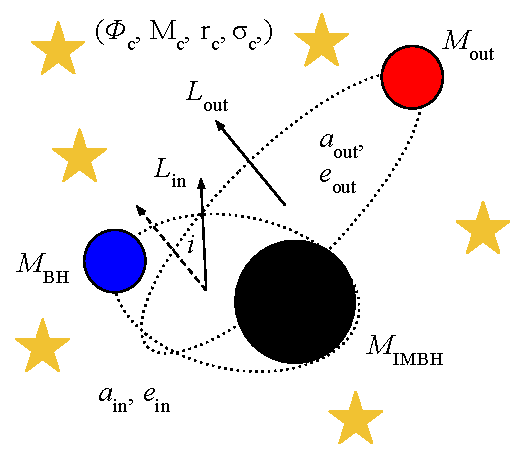
\includegraphics[width=7cm]{triple}
    \caption{Sketch of the IMBH-BH-BH triple configuration.}
    \label{fig:f1}
\end{figure}

Therefore, the phase space that characterises the triple's main properties can be dissected into three groups:
\begin{itemize}
    \item {\bf Inner binary (IMBH+BH)}: depends on the IMBH and BH masses, $M_\ibh$ and $M_\bhu$, the binary semi-major axis $a_\inn$ and its eccentricity $e_\inn$.
    \item {\bf Outer binary (IMBH+BH+BH)}: depends on the third BH mass, $M_\bhd$, semi-major axis $a_\out$, eccentricity $e_\out$.
    \item {\bf Host cluster}: we model the host cluster as a \cite{Deh93} sphere, characterized by total mass, $M_\gc$, scale radius, $r_\gc$, and the inner slope of the density profile $\gamma$.
\end{itemize}

In order to unveil the link between IMRIs formation and IMBH properties, we select the IMBH mass among eight different values ${\rm Log}(M_\ibh/\Ms) = 2-2.5-3-3.5-4-4.5-5-5.5$. This range covers typical values of putative IMBH masses forming in stellar systems of various sizes, from young and open clusters, to globular clusters, and up to low-mass nuclear clusters and dwarf galaxies.

Stellar BH masses are selected between $M_{\rm min} = 10\Ms$ and $M_{\rm max} = 30\Ms$, a mass range typical of stellar environments with a metallicity $Z<0.25\Zs$ \citep{belczynski16,spera16}. 
From Figure 5 of \cite{belczynski16}, we find that the BH mass can be connected to the initial star mass via a simple power-law 
\begin{equation}
\left(\frac{m_\bh}{\Ms}\right) = A(Z) \left(\frac{m_*}{\Ms}\right)^{C(Z)} + B(Z),
\end{equation}
with the coefficient depending on the metallicity as summarized in Table \ref{tab:t1}.

Assuming that BH progenitor stars follow initially a standard \cite{kroupa01} initial mass function, $f(m_*) \propto m_*^-s$, we can infer BHs final mass distribution simply as $f(m_\bh)\propto m_\bh^{-s/C(Z)}$. This simple approximation leads to a slope $s/C(Z) = 1.71-1.92$. 

However, we must take into account the fact that during clusters' early evolutionary stages stellar BHs sink into the centre due to mass segregation and start interacting strongly among each other.
As interactions take place, the heaviest BHs are expected to be either kicked out or accreted onto the IMBH seed \citep{giersz15,AAG18a}, potentially causing a strong depletion of BHs especially in the high-end tail of the mass distribution. We assume that the probability for a BH to be ejected or consumed in a merger scales with a weak power of the BH mass, namely $ \propto m_\bh^0.5$. Although quite arbitrary, such choice serves to account for the crucial role played by BHs interactions during the phases that contribute to the IMBH buildup. Given the assumptions above, our models are characterized by a mass function with total slope $\delta_\bh = -2.2$.

\begin{table}
    \centering
    \caption{Stellar - BH mass relation}
    \begin{tabular}{cccc}
        \hline
        \hline
        $Z$ & $A$ & $B$ & $C$ \\
        $\Zs$   &  & &  \\
    \hline    
        $0.005 $& $0.076\pm0.008$ & $3.8\pm0.3$ & $1.35\pm0.02$\\
        $0.25$  & $0.11\pm0.04$   & $0  $       & $1.20\pm0.07$\\
    \hline
    \end{tabular}
    \label{tab:t1}
\end{table}

Inner binary semi-major axis, $a_\inn$, is selected according to a distribution flat in logarithmic values, limited between $10$ and $315$ AU. Same distribution is assumed for the outer binary, but in this case $a_\out$ is chosen in two different ranges, either $a_\out=20-630$ AU or $630-1580$ AU. As detailed below, these ranges characterize two sets of simulations.
The eccentricity is assumed to follow a thermal distribution \citep{jeans19}, $P(e){\rm d}e = 2e{\rm d}e$ for both inner ($e_\inn$) and outer ($e_\out$) binary.

The cosine of the mutual orbital inclination between the inner and outer orbit, $\cos(i)$ is selected randomly between $-1$ and $1$.

The host cluster is assumed to be described by a \cite{Deh93} sphere, characterized by 
total mass $M_\gc$, scale radius $r_\gc$ and slope of the density profile $\gamma$.
The cluster length scale $r_\gc$ is selected randomly between 0.2 and 1.0 pc. For the cluster density slope, we assume a flat distribution with upper limit $\gamma \leq 1$.
To assign clusters' mass we either assume a scaling relation between the IMBH and the cluster mass, $M_\ibh - M_\gc$, or between the IMBH mass and the cluster velocity dispersion, $M_\ibh-\sigma_\gc$. 

In the first case, we take advantage of the scaling relations based on numerical models of IMBH formation and observations of putative IMBHs in globular clusters \citep{zwart02,Lutzgendorf13,AS16}. In particular, we adopt the scaling provided by \cite{AS16}, connecting the host cluster mass $M_\gc$ with the total ''dark'' mass, inhabiting the cluster's centre, comprised of either an IMBH or a sizable population of stellar BHs
\begin{equation}
\Log \left(\frac{M_\gc}{\Ms}\right) = \alpha \Log \left(\frac{M_\ibh}{\Ms}\right) + \beta.
\label{mcmibh}
\end{equation}
with $\alpha = 0.999 \pm 0.001$ and $\beta = 2.23 \pm 0.009$. 

Similarly to super-massive BHs in galactic nuclei, we can define the IMBH influence radius $R_{\rm inf}$, which delimits the region of space where IMBH dominates dynamics. This quantity can be connected to the cluster structural properties, namely
 \begin{equation}
 R_{\rm inf} = \frac{GM_\ibh}{\sigma_\gc^2} = \frac{M_\ibh}{M_\gc}R_{\rm hm},
 \end{equation}
 where we substituted the cluster velocity dispersion $\sigma_\gc$ with its value calculated at the cluster half-mass radius $R_{\rm hm}$, which in turn can be expressed in terms of the length scale and slope as
\begin{equation}
R_{\rm hm} = r_\gc(2^{1/(3-\gamma)}-1)^{-1}.
\end{equation} 
Combining the two equations above lead to 
\begin{equation}
R_{\rm inf} = \mu r_\gc(2^{1/(3-\gamma)}-1)^{-1},
\end{equation}
where $\mu = M_\ibh/M_\gc = 0.0058$ via Equation \ref{mcmibh}, thus implying that the the IMBH sphere of influence depends only on the cluster scale length and density slope. 

In the second case, instead, we assume that GCs central regions represent a downsized version of galactic nuclei, thus the IMBH mass can be connected to the velocity dispersion inverting the so-called $M_\ibh - \sigma_\gc$ relation as 
\begin{equation}
     \Log \left(\frac{\sigma_\gc}{200{\rm km~s}^{-1}}\right) = \frac{1}{\alpha}\left(\left(\frac{\Log M_\ibh}{\Ms}\right) - \beta\right) ,
\end{equation}
with $\alpha = 4.24\pm0.41$ and $\beta=8.12\pm 0.08$ \citep{gultekin09}. Additionally, we associate to the cluster randomly a concentration parameter $c$ between $10.7$ and $131.4$, a range of values typical of dense star clusters characterized by an adimensional potential well $W_0 = 6-9$ \citep{king62}. The cluster mass is then calculated as $M_\gc = 2\sigma_\gc^2 c r_\gc / G$.

We develop three simulations sets, depending on the allowed range for $a_\out$ and the relation assumed to connect the IMBH and host cluster properties. For each set, we run a total of 2000 simulations equally distributed among 8 IMBH mass bins. Therefore, for each value of $M_\ibh$ we gather 250 simulations. The main properties of our runs are summarized in Table \ref{tab:t2}.

Our simulations are performed taking advantage of \ARGdf \citep{ASCD19}, a modified version of \ARCHAIN that implements post-Newtonian dynamics up to order 2.5 and {\it algorithmic regularization} to handle close encounters and strong collisions \citep{mikkola99,mikkola08}. Additionally, \ARGdf allows the user to take into account in particles' equations of motion the gravitational field generated by the host stellary system and a dynamical friction term. Simulations are halted either if one of the two BH merge with the IMBH, if one of the BHs is ejected away of if the simulated time exceeds $t = 10^3 P_{\rm max}$, where $P_{\rm max}$ identifies the maximum between the inner and outer binary orbital period.

\begin{table*}
\begin{center}
\caption{Main properties of our models}
\begin{tabular}{cccccccccc}
\hline
model   & $M_\ibh$ & $\delta_\bh$ & $M_\bh$ & $a_\inn$ & $a_\out$ & $P(e)$ &$P(\cos(i))$ &Cluster scaling & $N_{\rm sim}$\\ 
        & $\Ms$    &            & $\Ms$   & $\au$    &  $\au$    &         &  &relation &\\
\hline 
0 & $10^2-5\times 10^5$ & $-2.2$ & $10-30$ & $10-315$ & $20-630$ & $2e$ & const&$M_\ibh -M_\gc$ & 2000\\
1 & $10^2-5\times 10^5$ & $-2.2$ & $10-30$ & $10-315$ & $20-630$ & $2e$ & const&$M_\ibh -\sigma_\gc$ & 2000\\
2 & $10^2-5\times 10^5$ & $-2.2$ & $10-30$ & $10-315$ & $630-1580$ & $2e$ &const &$M_\ibh -M_\gc$ & 2000\\
\hline
\end{tabular}
\begin{tablenotes}
\item Col. 1: model ID. Col. 2: mass of the IMBH, we adopt a sampling flat in logarithmic values. Col. 3: slope of the BH mass function adopted. Col. 4: range of masses adopted for stellar BHs. Col. 5-6: range of initial values for the inner/outer semimajor axis, we adopt a sampling flat in  logarithmic values. Col. 7-8: adopted distribution for initial eccentricity/inclination. Col. 9: adopted scaling to connect the IMBH and the cluster masses. Col. 10: Number of simulations performed.
\end{tablenotes}
\end{center}
\label{tab:t2}
\end{table*}



\section{Results}
\label{res}


\subsection{IMRIs formation channels and subsequent evolution}
\label{sec:imris}
The evolution of the IMBH-BH-BH triple immersed in the host cluster gravitational field can lead to very different outcomes, as shown in Figure \ref{fig:f3}:
\begin{itemize}
    \item {\bf Disrupted triple.} The three-body interaction undergoes a chaotic phases that ultimately lead to the ejection of a stellar BHs, whereas the inner binary either preserves its original components or undergoes a component swap.
    \item {\bf Stable triple.} The triple arranges in a configuration that satisfies the stability criterion for three-body systems. 
	\begin{itemize}
		\item {\bf Hierarchical triple.}  The triple arranges in a hierarchical configuration, with the outer BHs perturbing secularly the evolution of the inner binary. In this case, the inner binary can develop Kozai-Lidov oscillations \citep{kozai62,lidov62} that can trigger its eccentricity to grow to values close to unity. 
	\end{itemize}
    \item {\bf Unstable triple.} The inner and outer binary are in an unstable configuration, whose evolution is mostly dominated by chaos.
\end{itemize}

\begin{figure*}
    \centering
    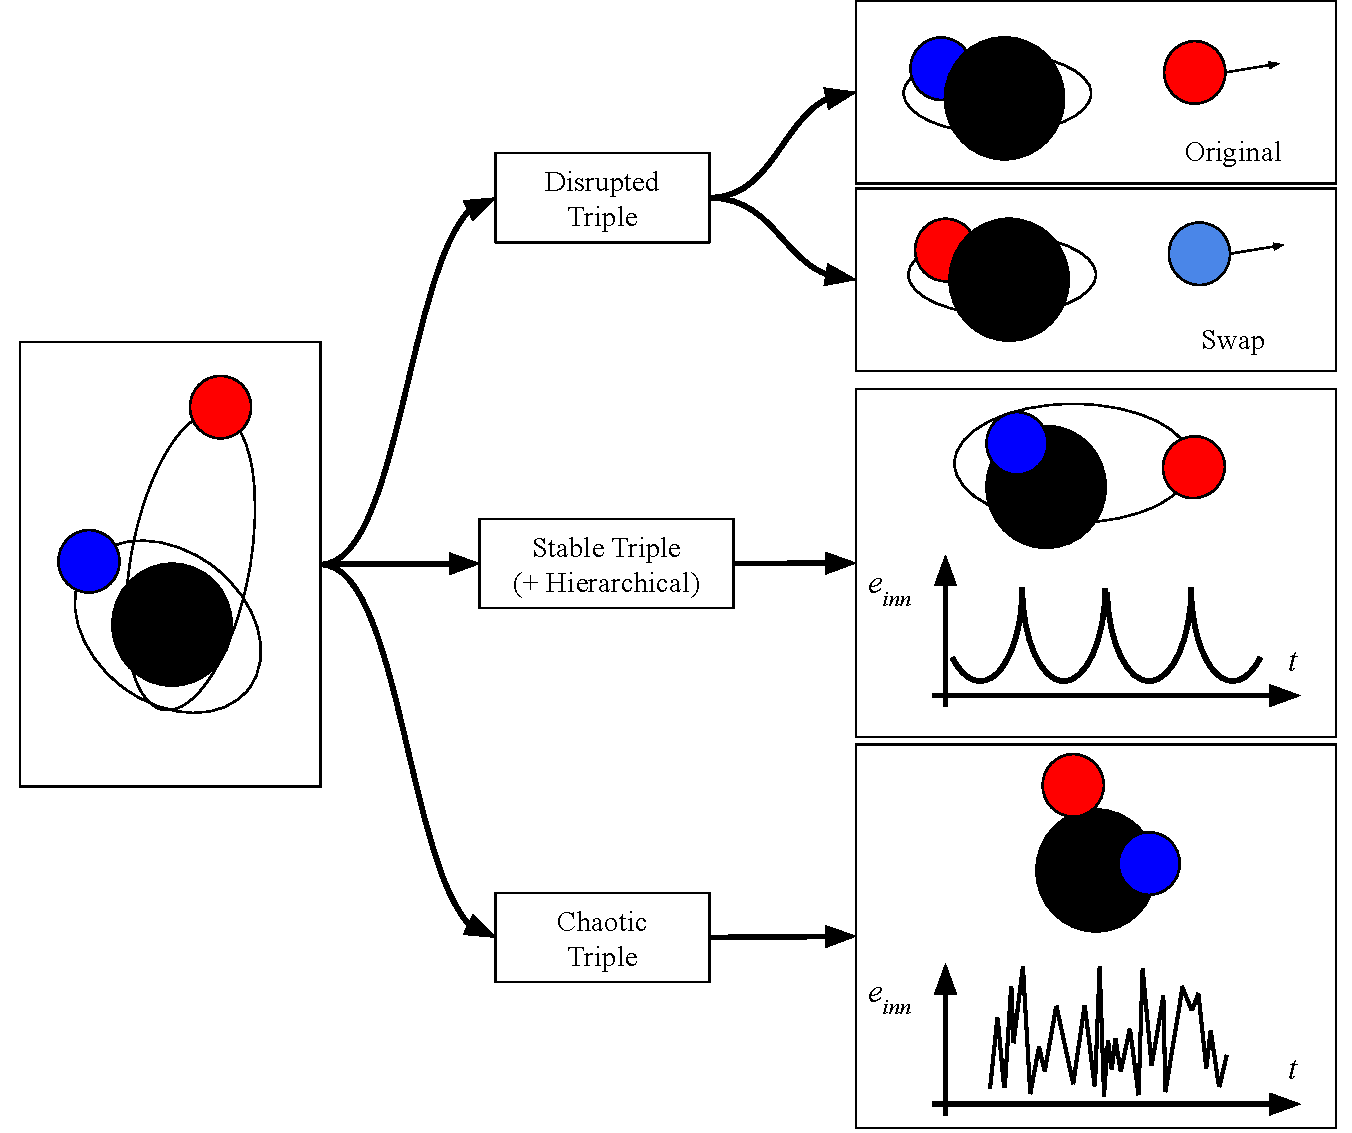
\includegraphics[width=16cm]{Sketch_IMRI}
    \caption{Schematic view of IMBH-BH-BH triple evolution.}
    \label{fig:f3}
\end{figure*}

In case of BH ejection, the evolution of remaining IMBH-BH will be due to the sum of two contributes, namely energy removal from binary-single interactions and GW emission. If the IMBH-BH entered the IMRI phase, binary-single interactions are expected to play little to no effect on its evolution \citep{seoane18}. In this case, the IMRI will continuously shrink emitting GW until coalescence, which takes place on a timescale \citep{peters64}
\begin{align}
t_\gw =&  \displaystyle \frac{5}{256}\frac{c^5 a_\inn^4 (1-e_\inn^2)^{7/2}}{G^3M_\ibh M_\bh(M_\ibh+M_\bh)} = \nonumber \\
       & 10^6{\rm ~yr}\left(\frac{a_\inn}{0.1\au}\right)^4\left(1-e_\inn^2\right)^{7/2}\times \nonumber \\ 
       & \times \left(\frac{10^3\Ms}{M_\ibh}\right) \left(\frac{30\Ms}{M_\bh}\right)\left(\frac{1030\Ms}{M_\ibh+M_\bh}\right).
\label{peters}
\end{align}

We note that for circular IMBH-BH binary in our model ($a_\inn=10\au$) the corresponding merger timescale is $t_\gw \sim 10^{14}$ yr, thus implying that some external perturbation is needed to trigger IMRI formation within a Hubble time.

In the second case, the triple is dynamically stable and the effects of perturbations arising from one of the component emerges secularly.  According to the \cite{mardling01} criterion, a triple is stable if
\begin{equation}
    \frac{a_\out}{a_\inn} > \frac{2.8}{1-e_\out}\left(1-\frac{0.3i}{\pi}\right)\left[\frac{(1+q_\out)(1+e_\out}{\sqrt{1-e_\out}}\right]^{2/5}, 
\label{stabcri}
\end{equation}
being $q_\out = m_\out/(m_\imbh + m_\bh)$.

If the triple arranges in a hierarchical configuration, its evolution can be dominated by secular perturbations known as Kozai-Lidov \citep{kozai62,lidov62}, which can induce periodic oscillations in the mutual inclination and the inner binary eccentricity. A parameter widely used to discern hierarchical triples is defined as \citep{Lithwick11,naoz11}
\begin{equation}
\epsilon_\kl = \frac{M_\imbh - m_\bh }{M_\imbh + m_\bh} \frac{a_{\inn}}{a_{\out}}\frac{e_{\out}}{(1-e_{\out}^2)},
\end{equation}
being the triple hierarchical if $|\epsilon| > 0.01$.

In this configuration, the eccentricity can increase up to values close to unity \citep{naoz11,naoz16}, leading the inner binary to continuously lose energy via bursts of GWs emitted at each pericentral passage. Therefore, the periodic eccentricity increase can drive the inner binary into the GW emission-dominated regime and trigger the formation of the IMRI. Kozai-Lidov oscillations cause a reduction of the merging timescale \citep[see for instance]{antonini12}
\begin{equation}
    t_{\rm gwKL} = \frac{t_\gw}{\sqrt{1-e_{\rm max}^2}},
\label{kozai}
\end{equation}
being $e_{\rm max}$ the maximum eccentricity achieved by the inner binary. 

In the case of an unstable triple, the inner and outer binaries have similar orbital properties and dynamics is mostly dominated by chaotic interactions.

In our models, we calculate $\epsilon_\kl$ and $a_\out/a_\inn$ at the end of the simulations, in order to identify to which category a triple belongs. 
In the case of models categorized as ``Disrupted'', the merger time is calculated simply via 
Equation \ref{peters}. For ``Hierarchical'' models, instead, we adopt Equation \ref{kozai}. Finally, for both ``Stable'' and ``Unstable'' models, the merger time is inferred as the average of the initial and final merger time and the same quantity evaluated in correspondence of the maximum eccentricity. Note that for ``Stable'' triples the merger time does not change dramatically over the simulated time.

\subsection{IMRIs properties}

We mark as IMRI candidates all IMBH-BH that, by the end of the simulations, have a merger time below 13 Gyr. 

We find quite similar results in both SET0 and SET1, thus implying that both the host cluster mass does not change significantly from one method to the other, and that the external potential has a little effect on the triple evolution. The latter is due to the fact that we are looking in the immediate cluster centre vicinity, where dynamics is dominated by the IMBH.

In SET0, an IMRI develop in $259$ cases out of 2000, i.e. $f_{\rm mer} = 12.95\%$ of formation probability. Concerning the formation channel, $6.6\%$ of IMRIs formed from Disrupted, $61.4\%$ from Stable, and $32\%$ from Hierarchical. Similarly, in SET1 we find $312$ IMRIs ($15.6\%$), $4.2\%$ of them formed from Disrupted, $62.8\%$ from Stable triples, and $33\%$ from Hierarchical. In SET2, we still find a similar merger probability ($f_{\rm mer} = 15.36\%$), but in this case the number of Hierarchical configurations outnumbers the other class of merger candidates covering the $83.7\%$ of the whole merger population. This is due to the fact that a larger outer semiaxis makes easier to satisfy the stability criterion in Equation \ref{stabcri}.
All IMRIs formation probability for different channels are summarized in Table \ref{tab:t3}. 

\begin{table}
    \centering
    \caption{IMRIs formation probability}
    \begin{tabular}{cccccc}
        \hline
        \hline 
        model& $f_{\rm mer}$ & $f_{\rm mer,D}$ & $f_{\rm mer,U}$ & $f_{\rm mer,H}$\\
             & $\%$& $\%$& $\%$& $\%$\\
        \hline
		SET0 & $12.95$ & $6.6$ & $61.4$ & $32$ \\
		SET1 & $15.60$ & $4.2$ & $62.8$ & $33$ \\
		SET2 & $15.36$ & $2.3$ & $14$   & $83.7$ \\
        \hline
    \end{tabular}
    \label{tab:t3}
\end{table}


Figure \ref{fig:f4} shows a comparison between the initial and final distribution of IMRI candidates' semi-major axis and eccentricity. We stress that both $a_\inn$ and $e_\inn$ are calculated from the last snapshot, thus they do not necessarily represent the binary orbital parameters promptly before the mergers. We postpone the discussion on the last stages of the IMRIs evolution to the next section.

The top panel shows clearly that the semi-major axis distribution of merging binaries differs significantly from the initial values, which is nearly uniform in the logarithms by assumption. The final distribution shows a peak at $\sim 10\au$, with a low-end extending down to $\lesssim 0.1 \au$. The eccentricity distribution, which is shown in the bottom panel, highlights that merging binaries tend to have a distribution steeper than the initial, thus implying that merger candidates are characterised by high eccentricities. Note that these distribution does not differentiate models with a different IMBH mass. 

\begin{figure}
\centering
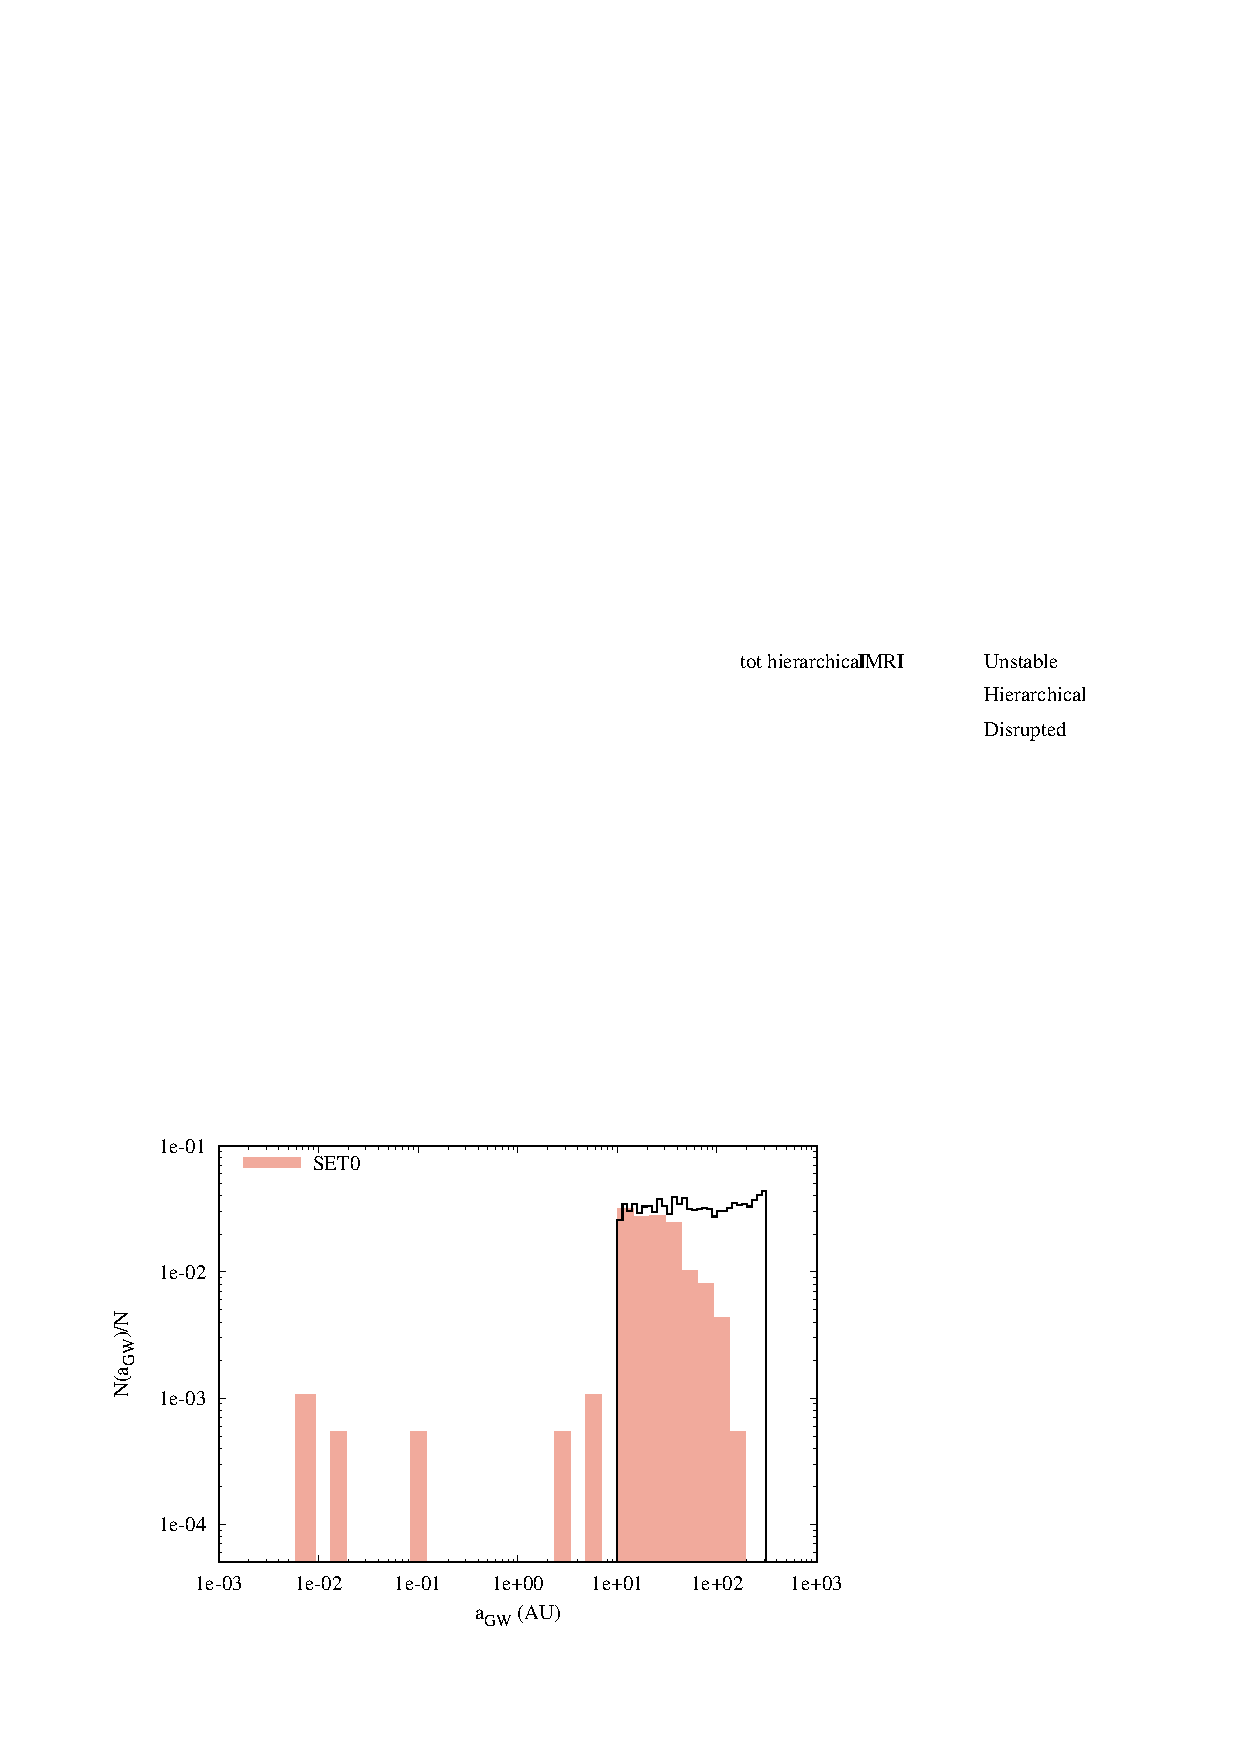
\includegraphics[width=\columnwidth]{semiaxis}\\
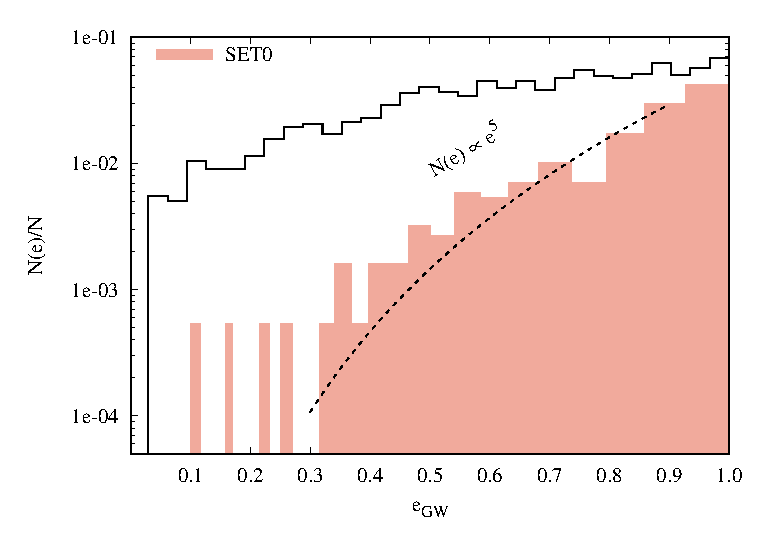
\includegraphics[width=\columnwidth]{ecce}
\caption{Top panel: semi-major axis distribution for the inner binary. The black steps refer to initial values for all the simulations performed, while the red filled steps refer only to merger binaries and final values. Bottom panel: the same as in top panel, but for the inner binary eccentricity.}
\label{fig:f4}
\end{figure}

\subsection{The role of the IMBH mass}

To explore the dependence between IMRI candidates eccentricity at formation and IMBH mass, we take the eccentricity directly from the last snapshot for models targeted as ``Disrupted'' and ``Unstable'', while for ``Hierarchical'' we record the maximum eccentricity. We then calculate the mean eccentricity value $\langle e_\gw\rangle$  in different mass bins, making the same for the subset of IMRI candidates, as shown in Figure \ref{fig:f4}. In general, it seems that, regardless of the set, IMRI candidates with masses below $5\times10^3\Ms$ have, on average, $\langle e_\gw\rangle$ larger compared to the whole simulations sample, while this trend reverses for heavier IMRIs. 
The average eccentricity increases in the $10^2-5\times10^3\Ms$ mass range, peaking at around $500-1000\Ms$, and than decreases rapidly at increasing the IMBH mass.This implies that the evolution of the inner binary leads the eccentricity to achieve larger values in correspondence of lighter IMBHs. We find that IMBHs with masses typical of star clusters $10^3<M_\ibh/\Ms<10^4$ are expected to form, on average, extremely eccentric IMRIs, while the eccentricity at formation attains more moderate values at IMBH masses typical of low-mass dwarf galaxies and nuclear clusters.
While affecting the eccentricity, the IMBH mass does not have a significant effect on the companion BH mass. Indeed, IMRIs light component masses follows the assumed BH mass distribution. 

\begin{figure}
\centering
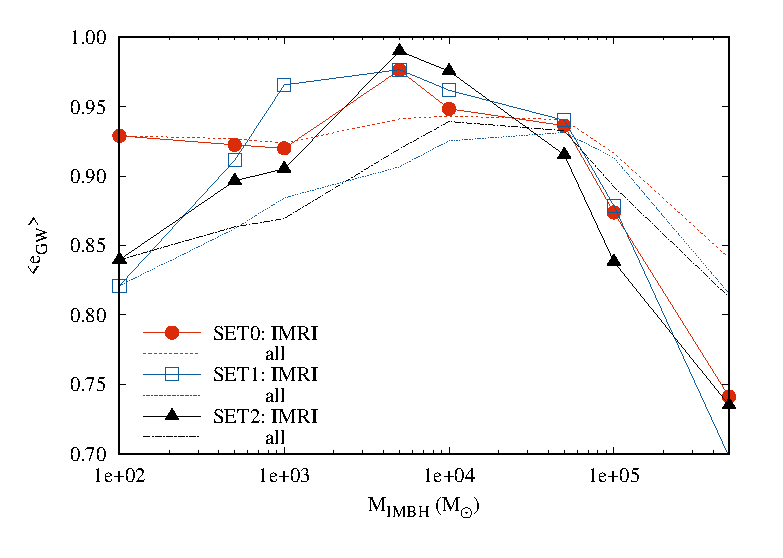
\includegraphics[width=\columnwidth]{average_ecc_sets}\\
\caption{The average eccentricity ($\langle e_{\rm mer}\rangle$), calculated at the end of simulaitons in different IMBH mass bins, as a function of the IMBH mass and for different sets. We show the IMRIs average eccentricity SET0 (filled red points), SET1 (open blue squares), and SET2 (filled black points). The total average value is also marked for SET0 (dashed red line), SET1 (dotted blue line), and SET2 (dot-dashed black line). }
\label{fig:f5}
\end{figure}

The merger times associated with IMRIs show a broad distribution regardless of the models set considered. Figure \ref{fig:f6} shows the cumulative distribution of $t_\gw$ calculated as discussed in Section \ref{sec:imris}.

\begin{figure}
\centering
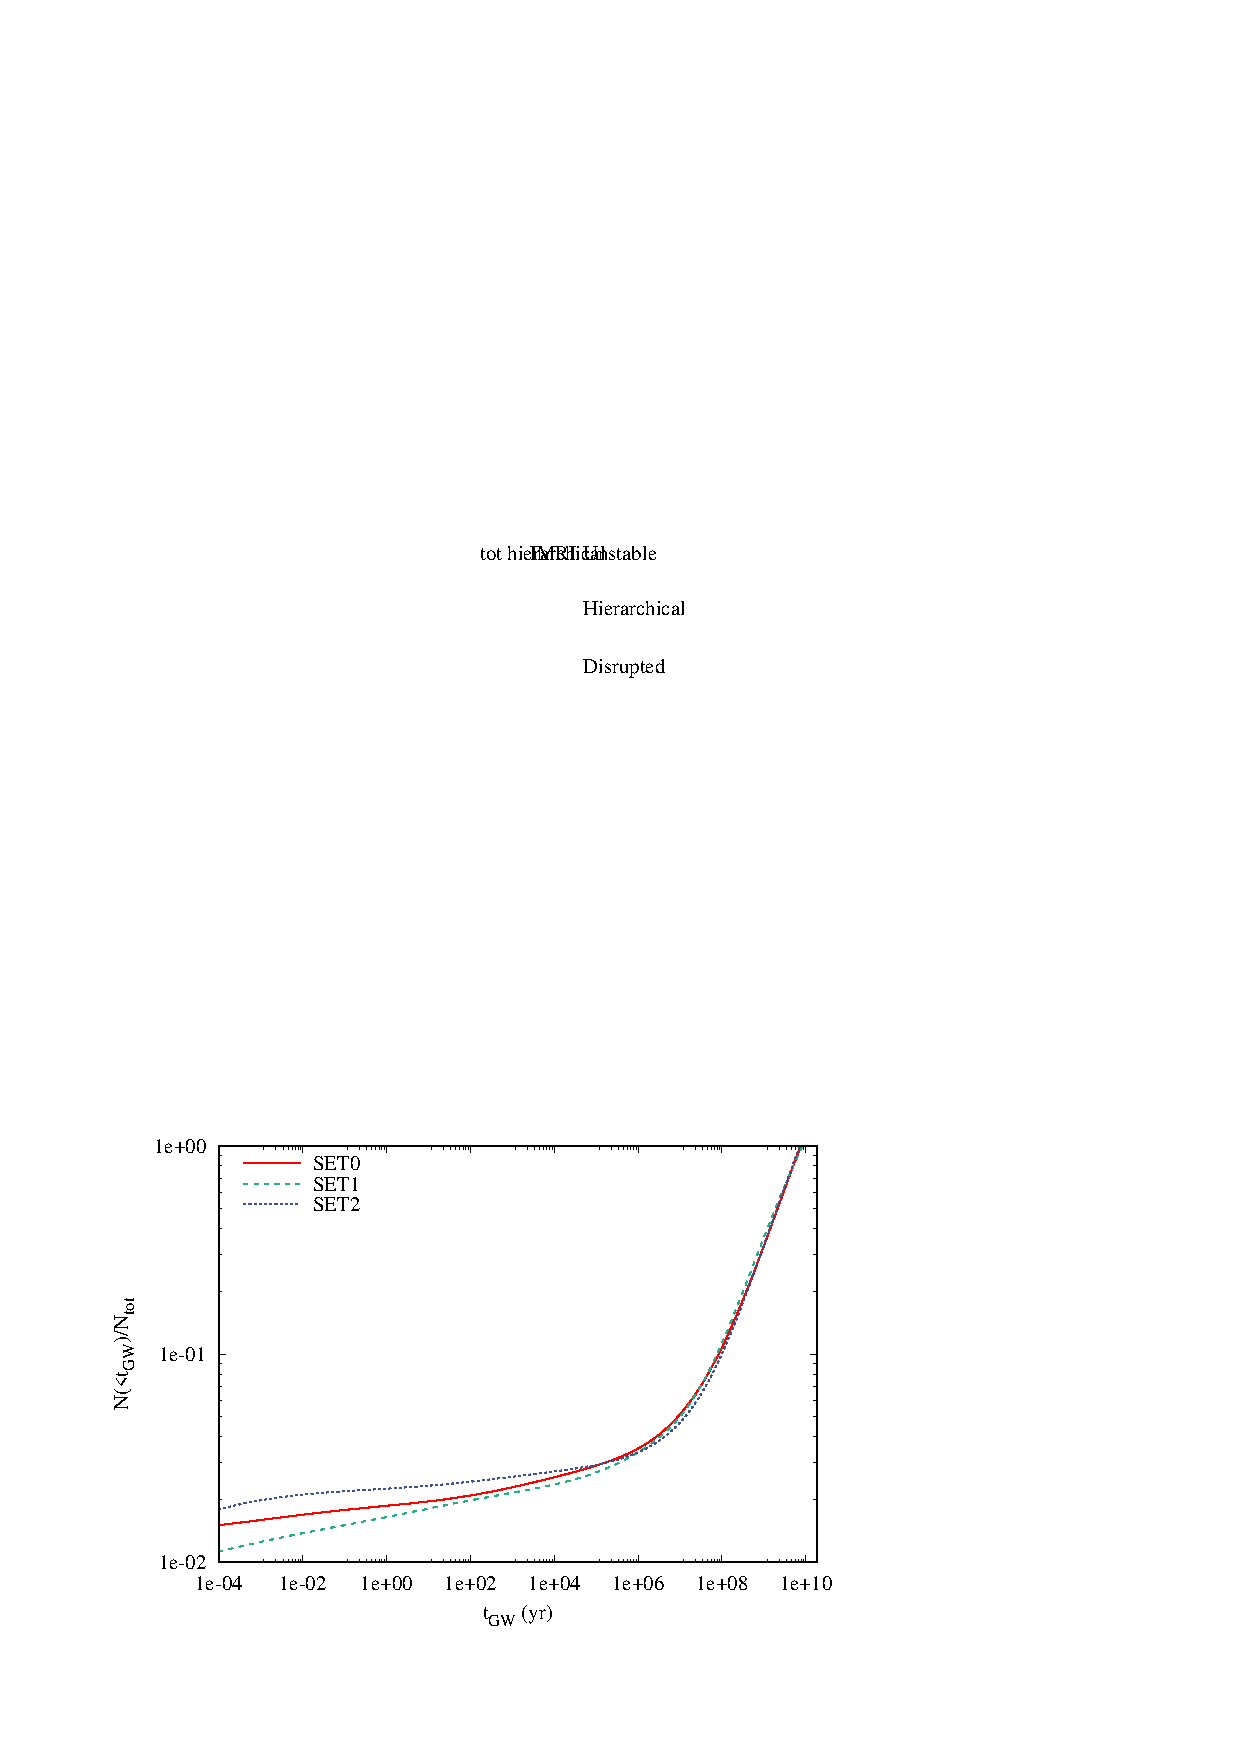
\includegraphics[width=\columnwidth]{TGW_distribution}
\caption{Cumulative distribution of IMRI merger times for all the models investigated.}
\label{fig:f6}
\end{figure}

In order to uncover what is the role played by the IMBH in determining IMRIs formation, we calculate the percentage of IMRIs formed in different mass bins. This quantity, namely $f_{\rm mer}$, represents {\it de facto} IMRIs formation probability. We find that $f_{\rm mer}$ follows quite a precise trend, regardless of the set, thus in what follows we focus on SET0 only, for clarity's sake.

\begin{figure}
	\centering
    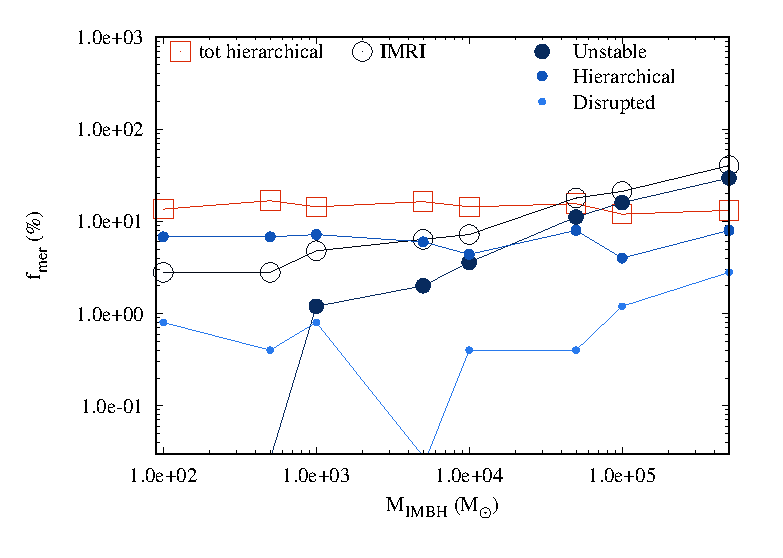
\includegraphics[width=\columnwidth]{mergers}
	\caption{IMRIs formation probability as a function of the IMBH mass for SET0. Red open squares shows all the models that are in an either stable or hierarchical configuration at the end of the simulation. Open dark blue circles identify IMRIs. From larger to smaller circles, blue filled circles represent IMRIs formed from unstable, hierarchical, and disrupted triples.}
	\label{fig:f7}
\end{figure}

Figure \ref{fig:f7} shows the $f_{\rm mer}-M_\ibh$ relation in the case of SET0. We differentiate between IMRIs forming in disrupted triples, in a hierarchical or unstable configuration. 
Our results suggest that an IMBH-BH-BH has a $10\%$ of probability to arrange in a hierarchical configuration, regardless of the IMBH mass or the GW timescale. IMRIs formation probability, instead, increases weakly with IMBH mass, increasing from $\sim 2\%$ for $M_\ibh \simeq 10^2$ to up to $15\%$ for heavy IMBH, $M_\ibh>10^5\Ms$.

At IMBH mass values below $10^4\Ms$, we find that Hierarchical and Unstable systems contribute equally to the whole IMRI population, while at larger IMBH masses the majority of IMRIs is comprised of Unstable triples. IMRIs forming out of Disrupted triples give little contribution to the population, being their formation probability only $0.5-1\%$.

Figure \ref{fig:f8} shows how $f_{\rm mer}$ varies for the three set explored. In the IMBH mass range $M_\ibh>10^3\Ms$, this relation is well described by a simple powerlaw
\begin{equation}
f_{\rm mer} = \alpha \left(\frac{M_\ibh}{10^2\Ms}\right)^\beta,
\label{fmerg}
\end{equation}  
with $\alpha = (1.5\pm0.2)\times 10^{-2}$ and $\beta = 0.39\pm0.02$. 


\begin{figure}
    \centering
    \includegraphics[width=\columnwidth]{merger_sets.eps}
    \caption{IMRIs formation probability as a function of the IMBH mass for the three simulated sets.}
    \label{fig:f8}
\end{figure}

Our simulations suggest that whenever a three-body encounter occurs in a GC containing a $10^4\Ms$ IMBH, there is a $\sim 10\%$ of the probability for IMRIs formation and the eccentricity at formation is of the order of 0.95. 

\subsection{The serendipitous formation of stellar BH binaries around an IMBH}

Among all the runs performed, we find two interesting cases, namely s151 and s400, in which the stellar mass BHs are initially sufficiently close to form a tight binary. In both cases, the IMBH mass is relatively small $M_{\ibh} = 100\Ms$, and the inner binary is comprised of the other two, stellar-mass, BHs. It is not surprising that a BH-BH pair forms in a model with low-mass IMBH, due to the lower velocity dispersion and the larger tidal radius needed for the binary to form without being ripped apart from the IMBH. In both cases, the BH-BH binary undergoes Kozai-Lidov oscillations, which periodically induce an increase in the binary eccentricity and the mutual inclination.

In model s400, the amplitude of the oscillation is minimal, the mutual inclination ranges between $i = 126-130^\circ$, while the eccentricity varies in the range $e = 0.882-0.904$. Although the KL effect is not very efficient in affecting the BH-BH evolution, the binary is sufficiently tight to have a short merger timescale, being $t_{\rm gw} \simeq 3\times 10^7$ yr.

In model s151, instead, the Kozai-Lidov effect is more effective, leading the inclination to vary strongly in the range $\sim 40-90^\circ$ and the eccentricity to rise up to $e = 0.99$. The time evolution of both $e$ and $i$ is shown in Figure \ref{F9}, together with the associated merger time-scale. 
In this particular simulation, the reduction of the merger time related to the episodic GW emission as described in Equation \ref{kozai}, trigger the BH binary coalesce in a time $5600$ times smaller than the time needed for the same binary to merge in isolation.

In both the cases that we find, the IMBH mass is $M_\ibh=100\Ms$. Heavier IMBHs would make BH-BH pairing much harder, because of the higher velocity dispersion and the larger gravitational influence. Having 250 simulations with $M_\ibh=100\Ms$ in each set, we can infer BH-BH formation probability as $P_{\rm bhb} = 0.8\%$.

\begin{figure}
\centering 
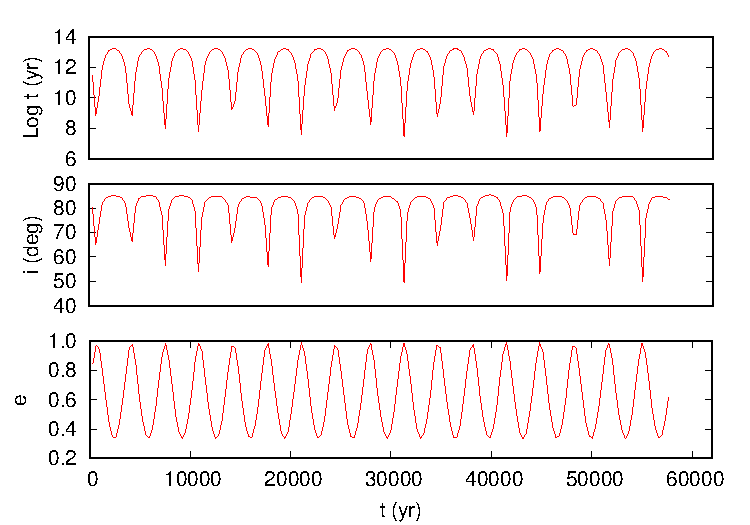
\includegraphics[width=\columnwidth]{kozai_151}
\caption{Top panel: time evolution of the merger timescale for model number 151, in which two BHs pair together while the IMBH acts as a perturber. Central panel: mutual inclination as a function of time for the BH-BH pair in simulation number 151. Bottom panel: ecentricity as a function of time for the BH-BH pair in simulation number 151.}
\label{F9}
\end{figure}


\subsection{IMRIs merger rate}

Previous studies based on full consistent N-body simulations of star clusters containing IMBHs with various masses and general properties  \citep{konstantinidis13,haster16,leigh14, macleod16} have shown that binary formation involving an IMBH takes place at a rate of $R_{\rm bin} \sim 10^{-7}$ yr. Assuming typical ages for globular-like star clusters of $t_{\rm age}\sim 10^{10}$ yr and assuming that IMBH buildup occurs in the clusters early lifetime ($\lesssim 1$ Gyr), we can use the merger probability fitting function depicted in Equation \ref{fmerg} to infer the total number of IMRIs formed for a given IMBH mass and over a cluster lifetime $t_{\rm age}$
\begin{equation}
    N_\gc(M_\ibh) = R_{\rm bin}t_{\rm age}f_{\rm mer} \sim 15\left(\frac{M_{\ibh}}{10^2\Ms}\right)^{0.38},
\end{equation}
ranging from $\Gamma_{\imri} = 15-90$ yr$^{-1}$ for $M_\ibh = 10^2-10^4\Ms$, respectively.
To put such a quantity in the context of MW-like galaxies, we need to make assumptions on the IMBH putative mass function. Assuming that the initial mass function of GCs follows a power-law and exploiting Equation \ref{mcmibh}, we can write the IMBH mass function as $f(M_\ibh) = k (M_\ibh/10^\alpha)^{1/beta}$. The normalization constant $k$ can be calculated by assuming that the mass in clusters constitute a fraction of the total galaxy mass:
\begin{equation}
k = \frac{\delta M_g (2-s)}{(M_{\gc 2}^{2-s} - M_{\gc 1}^{2-s})},
\label{normal}
\end{equation}
with $\delta = 5\times 10^{-4}$ \citep{webb15,belczinski17}, $M_g = 6\times 10^{10}\Ms$ and $M_{\gc 1,2} = (5\times 10^3 - 8\times 10^6)\Ms$ the range of GC initial masses allowed. 

%As recently suggested by \cite{AAG19}, out of the 151 Galactic GCs currently known, around 35 might be harbouring, at present time, an IMBH with mass in the range $10^3-10^4\Ms$. They find that the mass distribution of these putative IMBHs can be described by a Maxwellian in the form 
%\begin{equation}
%    f(x_\ibh) = \frac{a}{\sigma\sqrt(2\pi)}\exp{\left(-\frac{\left(x_\ibh - \mu\right)^2}{ (2\sigma^2)}\right)},
%\end{equation}
%with $x_\ibh\equiv \Log M_\ibh$, and $a=0.14\pm0.3$ , $\mu = 4.01\pm0.09$ and $\sigma = 0.4\pm0.1 $.
Combining equations above, we can infer the total number of IMRIs  MW-like galaxies as
\begin{align}
    N_{\rm MW} =& f_\ibh N_\gc \int_{M_{\ibh ,1}}^{M_{\ibh ,2}} \Gamma(M_\ibh) \times \nonumber \\
    & \times f(M_\ibh) \frac{\derd M_\gc}{\derd M_\ibh} {\rm d}M_\ibh,
\end{align}
where $f_\ibh N_\gc$ is the number of GCs containing an IMBH, and the term $\derd M_\gc / \derd M_\ibh$ is used to perform a change of variable from the GC to the IMBH mass. The integral has analytical solution in the form
\begin{equation}
N_{\rm MW} = K \frac{M_{\ibh ,2}^{\beta + b(1-s)} - M_{\ibh ,1}^{\beta + b(1-s)}}{\beta + b(1-s)},
\end{equation}
with the parameter $K$ containining all the constant factors.

%
%
%
% \frac{\Gamma_{\rm MW} (x_\ibh)}{f_\ibh N_\gc} =&   \frac{a}{2} (A + B\mu) {\rm erf}\left(\frac{x_\ibh-\mu}{\sigma\sqrt{2\pi}} \right) + \nonumber\\
%                                & - \frac{a}{\sqrt(2\pi)}B \sigma \exp{\left(\frac{-\left(x_\ibh-\mu\right)^2}{2\sigma^2}\right)},
%\end{align}
% the coefficients $A = \alpha - \beta\ln(100)$ and $B \equiv \beta$ are conveniently manipulated from Equation \ref{fmerg}.
%Assuming a typical IMBH population spanning the mass range $10^2-10^4\Ms$, a number of GCs $N_\gc = 151$, a fraction $f_\ibh \simeq 35/151$ of GCs hosting an IMBH we can infer the MW-IMRI rate 
%\begin{equation}
%\Gamma_{\rm MW,IMRI} \simeq 4\times 10^{-3} {\rm MW}^{-1} {\rm yr}^{-1}
%\end{equation}
Assuming $t_{\rm age} = 10$ Gyr and in the IMBH mass range of $10^2 - 10^4\Ms$, we derive an IMRI merger rates for MW-like galaxies of
\begin{equation}
\Gamma_{\rm MW} = 2.26\times 10^{-5} {\rm ~yr} \left(\frac{10{\rm ~Gyr}}{t_{\rm age}}\right)\left(\frac{f_\ibh}{0.2}\right)\left(\frac{N_\gc}{180}\right).
\end{equation}
The number of MW-analogs in the local Universe (redshift $z<0.1$) is roughly proportional to the luminosity distance $D_L$, namely $P_{\rm MW} = 4\pi/3 \times 0.0116(2.26)^{-3}D_L^3$ with $D_L$ expressed in Mpc \citep{abadie10}. Thus a rough estimate of potential IMRIs developing in MW-like galaxies in the local Universe is given by $\Gamma_{\rm MW} \times P_{\rm MW} = 10.5$ yr$^{-1}$.
This is a simple estimate, though, which not account for the distribution of galaxies across different redshift or the actual volume within which a detector is sensitive.
The launch of the LISA detector and the start of operations of the next generation of GW observatories like the Einstein Telescope (ET) will enable us to observe this kind of objects at cosmological distances. Therefore, to infer the IMRI merger rates, we need to take into account in our calculation how the number density of galaxies varies across redshift $z$.
The GW source {\it horizon} determines the maximum distance in space, or the redshift $z_{\rm hor}$, at which the source signal is detected with a threshold signal-to-noise ratio (SNR), namely:
\begin{equation}
{\rm SNR^2} = \int_{f_1}^{f_2} \displaystyle{\frac{h_c^2(f,z_{\rm hor})}{S_n^2(f)}} {\rm d}f,
\end{equation}
with $f_{1,2}$ the initial and final frequency of the GW signal, $h_c(f,z)$ its characteristic strain, and $S_n(f)$ its sensitivity. To determine this quantity, we integrate the final stage of the IMRI signal assuming an observation time of 4 yr -- i.e. the nominal duration time of the LISA mission -- and we calculate the value of $z_{\rm hor}$ at which we get an SNR of 15. We assume the set of cosmological parameters measured by the Planck mission, namely $H_0 = 67.74$ km/s/Mpc$^{3}$, $\Omega_m = 0.3089$, $\Omega_\Lambda = 0.6911$ \citep{planck15}. To calculate $z_{\rm hor}$, we vary the IMBH mass in the range $50-10^6\Ms$ assuming that the companion has a mass of either $10$ or $30\Ms$. Figure \ref{fig:fhor} shows how the horizon redshift changes for four different detectors: the Laser Interferometer Space Antenna \citep[LISA\footnote{\url{https://www.elisascience.org/}},][]{amaro12}, the Deciherz Gravitational-Wave Observatory \citep[DECIGO\footnote{\url{http://tamago.mtk.nao.ac.jp/spacetime/decigo_e.html}},][]{seto01}, the Einstein Telescope \citep[ET\footnote{\url{http://www.et-gw.eu/}},][]{punturo10}, and LIGO. 


\begin{figure}
\centering
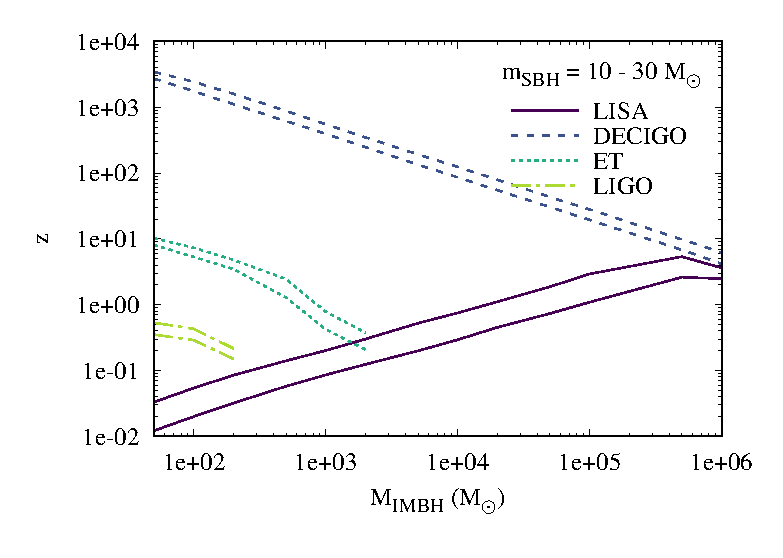
\includegraphics[width=\columnwidth]{horizon_IMBH}
\caption{Horizon redshift as a function of the IMBH mass assuming a BH companion with mass $10 \Ms$ (lower curves) or $30\Ms$ (upper curves). Different curve collections correspond to different detectors: LISA (straight lines), DECIGO (dashed lines), ET (dotted lines), LIGO (dot-dashed lines). }
\label{fig:fhor}
\end{figure}

From the plot is evident that ground based telescopes provide a relatively limited view on the IMBH realm, although LIGO can provide insights on low-mass IMRIs ($<500\Ms$) up to redshift $z_{\rm hor} = $ and ET will enable the observation of IMRIs with mass $<10^3\Ms$ up to $z_{\rm hor} = 1-10$, the same range of redshift accessible with LISA to listen GWs from heavy IMRIs ($M_{\imri}>10^4\Ms$). Decihertz observatories like DECIGO \citep{KawamuraEtAl2011} and similarly designed mission \citep{arca19}, instead, will allow the detection of IMRIs in the whole $50-10^6\Ms$ mass range up to the dawn of the Universe, thus constituting ideal detectors to unveil the truly nature of IMBHs. 

Once that the dependence between the horizon redshift and the IMBH mass is determined, we can infer the IMRIs rate by calculating the total number of IMRIs inside the cosmological volume encompassed by $z_{\rm hor}$, a requirement that can be expressed as:
\begin{align}
\Gamma_{\imri} = & \Omega_s \int_{M_{\ibh ,1}}^{M_{\ibh ,2}} \int_{0}^{z_{\rm hor}} \frac{\derd n_{\imri}}{\derd M_\ibh\derd z} \times \nonumber \\
& \times \frac{\derd V_c}{\derd z}  \derd z \derd M_\ibh,
\end{align}
being $\derd V_c/\derd z$ the comoving cosmological volume element, $\xi(M_\ibh)$ the IMBH mass function, and $\derd n_{\imri}/\derd M_\ibh$ the number of IMRIs per unit of IMBH mass. We can write the latter quantity as
\begin{align}
\frac{\derd n_{\imri}}{\derd M_\ibh} =& f_{\imri}(M_\ibh) p_\ibh e_{\imri}\times \nonumber \\
& \times \frac{\derd n}{\derd M_g\derd z}\frac{\derd n_\gc}{\derd M_\gc}\frac{\derd M_\gc}{\derd M_\ibh}.
\end{align}
Here, $\derd n/(\derd M_g \derd z)$ represents the number of galaxies per unit of redshift and galaxy mass, $\derd n/\derd M_\gc$ is the number of clusters per cluster mass in a given galaxy, $\derd M_\gc/\derd M_\ibh$ connects GCs and IMBHs, $e_\imri$ is the number of times that the same IMBH can form an IMRI with a stellar companion, $f_{\imri}(M_\ibh)$ is the fraction of IMRIs that undergo merger within a Hubble time (a quantity that is extracted from our simulations), and $p_\ibh$ represents the probability for a cluster to host an IMBH. In the following, we assume $p_\ibh = 0.2$ \citep{giersz15}.

The term $\derd M_\gc / \derd M_\ibh$ can be calculated by inverting Equation \ref{mcmibh} and performing the derative. For the number distribution of the GCs mass in a given galaxy, $\derd n/\derd M_\gc$, we assume a power-law
\begin{equation}
\frac{\derd n}{\derd M_\gc} = k M_\gc^{-s},
\end{equation}
with the slope $s = 2.2$ and the normalization constant given in Equation \ref{normal}. Following the previous calculations, we assume an average galaxy mass of $6\times 10^{10}\Ms$, and $M_{\gc 1,2} = (5\times 10^3 - 8\times 10^6) \Ms$, corresponding to an IMBH mass range $M_\ibh \simeq (30 - 4.6\times 10^4)\Ms$ according to Equation \ref{mcmibh}, which can also be used to write $M_\gc^{-s} = aM_\ibh^{-bs}$, with $a,b$ obtained manipulating conveniently the relation.
The $\derd n/(\derd M_g\derd z)$ is obtained exploiting the results in \cite{conselice16}, who studied the distribution of galaxies with stellar masses up to $10^{12}\Ms$ up to redshift $z=8$. In particular, we exploit the following parametric expression of galaxies number density 
\begin{equation}
\phi(z) = -\frac{\phi_* 10^{(\alpha_* + 1)(M_2-M_*)}}{\alpha_* + 1},
\end{equation}
with $\phi_*,~\alpha_*,~M_*$ depending on the redshift \citep[see Table 1 in][]{conselice16}, and $M_2 = 12$. 

Substituting all the terms and manipulating them conveniently, the total number of IMRI in the portion of Universe accessible to a given detector is thus given by
\begin{align}
N_{\imri,1} = & k a^{1-s} b p_\ibh e_\imri \times \nonumber \\
& \times \int_{M_{1}}^{M_{2}} \int_0^{z_{hor(M_\ibh)}} M_\ibh^{(1-s)b-1}  \times \nonumber \\
& \times  f_{\imri}(M_\ibh) \phi(z) \frac{\derd V_c}{\derd z} \derd z \derd M_\ibh.
\end{align}

Observations and models suggest that GCs formation peakes at redshift $z=2$, corresponding to a formation time of $t_{\gc ,f} = 3.285$ Gyr. This would imply that the maximum redshift at which a GC containing an IMBH can be observed is the maximum between the horizon redshift and the GC formation redshift. Even in the case in which we assume that GCs forms continuously, we need to set a maximum redshift above which stars did not form yet. We set $z = 6$, corresponding to the epoch of reionization. Thus, we capped the horizon redshift with either $z=2$ (peak of GC formation), or $z=6$ (formation of the first stars).

The time over which these IMRI forms can be estimated as the sum of the cluster formation time, the IMBH formation time, the IMRIs formation time, and the IMRI merger timescale:
\begin{equation}
T = t_{\gc ,f} + t_{\ibh ,f} + t_{\imri, f} + t_{\rm GW}. 
\end{equation}
The physics that regulate IMBH formation is still debated and partly unknown. Depending on the formation scenario, models suggest that the IMBH growth can occur either on short ($\sim 1$ Gyr) or long ($\simeq 5-10$ Gyr) timescales. As discussed recently, {\it fast} IMBHs could outnumber those forming slowly \citep{giersz15,AAG19}, thus in our calculations we assume $t_{\ibh ,f} = 2$ Gyr. 
The formation of an IMRI scales with the mass-segregation timescale in the host cluster, which is expected to be of the order of $\sim 0.1-1$ Gyr, while for $t_\gw$ we calculate, from our models, the value at which the number of mergers is half the total number, i.e. $N_\gw(t_\gw) = 0.5 N_\gw$. This corresponds to $t_\gw = 0.6-1.5$ Gyr. 

An alternative way, yet similar, to calculate the merger rate is by exploiting the cosmological GC star formation rate $\rho_{\rm SFR}(z)$, which can be used to calculate the total number of GCs at a given redshift
\begin{equation}
N(z_{\rm max}) = \frac{1}{<M_\gc>} \int_0^{z_{\rm max}} \rho_{\rm SFR}(z)\frac{\derd V_c}{\derd z}\derd z.
\end{equation} 
Given the power-law GCs mass function used in the previous method, the normalization factor in this case become
\begin{align}
k  =&\frac{(1-s)}{M_{\gc, 1}^{1-s} - M_{\gc ,2}^{1-s}},
\end{align}
and the total number of IMRI inside a given cosmological volume is thus given by
\begin{align}
N_{\imri, 2} = & k a^{1-s} b p_\ibh e_\imri \int_{M_{1}}^{M_{2}} \int_0^{z_{hor(M_\ibh)}} M_\ibh^{(1-s)b-1} \times \nonumber \\
& f_{\imri}(M_\ibh) N(z_{\rm max}) \frac{\derd V_c}{\derd z} \derd z \derd M_\ibh.
\end{align}


An estimate of the merger rate can therefore be calculated as $\Gamma_\imri = N_\imri / T$. 
Table \ref{tab:5} summarizes the merger rates calculated for different instruments, and assuming different parameters.

Our results suggest that LIGO can already be capable of observing up to $\sim 1.25-4.33$ mergers over a 4 yr observation involving IMRIs with a total mass $M_\imri = 40-230\Ms$ and mass ratio $M_\bh / M_\ibh = 0.05 - 1$ out to redshift $z = 0.15-0.57$. Over the same observation time, LISA would enable us to observe $\sim 1.9-30$ mergers with larger masses $M_\imri < 5\times 10^4\Ms$ and lower mass ratios, down to $q = 2\times 10^{-4}$, out to redshift $z \simeq 0.7-1.8$.

While the constraints on "present-day" technologies is already quite encouraging, the next generation of both ground- and spaced-observatories could provide quite a large amount of observation up to the maximum redshift allowed ($z=2-6$). Assuming a 4 yr observation mission, ET could detected up to $120-2600$ IMRIs per yr with masses $M_\imri < 2000 \Ms$. The space-based DECIGO could provide an even larger amount of observations per yr ($\sim 250-4400$ in 4 yr of observation), enabling the observation of IMRIs with total mass up to $\sim 5\times 10^4\Ms$ up to the epoch of GC formation and even up to the reionization epoch.


\begin{table*}
\caption{IMRI merger rate for different detectors}
\begin{center}
\begin{tabular}{cccccccc}
\hline
Instrument & $M_{\rm SBH}$ & $z_{\rm max}$ & $M_{\ibh ,1}$ & $M_{\ibh ,2}$ & $T$ & $\Gamma_1$ & $\Gamma_2$ \\
   & $\Ms$ & &$\Ms$ & $\Ms$ & Gyr & yr$^{-1}$ & yr$^{-1}$ \\ 
\hline
LIGO & $10$ & $0.38$ & $29$ & $200$ & $8$ & $1.25$ &$1.46$ \\
LIGO & $10$ & $0.38$ & $29$ & $200$ & $8$ & $1.25$ &$1.46$ \\
LIGO & $30$ & $0.57$ & $29$ & $200$ & $8$ & $3.00$ &$4.33$ \\
LIGO & $30$ & $0.57$ & $29$ & $200$ & $8$ & $3.00$ &$4.33$ \\
LISA & $10$ & $0.70$ & $29$ & $46240$ & $8$ & $1.90$ &$2.75$ \\
LISA & $10$ & $0.70$ & $29$ & $46240$ & $8$ & $1.90$ &$2.75$ \\
LISA & $30$ & $1.78$ & $29$ & $46240$ & $8$ & $29.34$ &$23.31$ \\
LISA & $30$ & $1.78$ & $29$ & $46240$ & $8$ & $29.34$ &$23.31$ \\
ET & $10$ & $2.00$ & $29$ & $2000$ & $8$ & $214.69$ &$123.87$ \\
ET & $10$ & $6.00$ & $29$ & $2000$ & $8$ & $2155.25$ &$396.60$ \\
ET & $30$ & $2.00$ & $29$ & $2000$ & $8$ & $238.18$ &$136.55$ \\
ET & $30$ & $6.00$ & $29$ & $2000$ & $8$ & $2571.14$ &$458.30$ \\
DECIGO & $10$ & $2.00$ & $29$ & $46240$ & $8$ & $357.06$ &$248.20$ \\
DECIGO & $10$ & $6.00$ & $29$ & $46240$ & $8$ & $4227.86$ &$996.72$ \\
DECIGO & $30$ & $2.00$ & $29$ & $46240$ & $8$ & $357.06$ &$248.20$ \\
DECIGO & $30$ & $6.00$ & $29$ & $46240$ & $8$ & $4227.86$ &$996.72$ \\
\hline
\label{tab:5}
\end{tabular}
\end{center}
\end{table*}




\section{Gravitational waves}

In this section we investigate the properties of IMRIs formed in our model from the perspective of GW emission. To perform our study, we take from the last snapshot of all the simulations the inner binary semi-major axis and either the maximum eccentricity, if the triple is marked as ``Hierarchical'', or the actual eccentricity, if the triple is marked as ``Disrupted'' or ``Unstable''.

In the following, we indicate semi-major axis and eccentricity with $a$ and $e$, respectively, while the IMRI mass is labelled with $M_{\rm bin}$.

As long as the binary preserve a residual eccentricity, the GW signal is audible in a range of frequency, rather than being monochromatic. The peak frequency can be approximated as \citep{wen03, antonini12}
\begin{equation}
f_\gw = \frac{1}{\pi}\sqrt{\frac{GM_{\rm bin}}{a^3}}\frac{\left(1+e\right)^{1.1954}}{\left(1-e^2\right)^{3/2}},
\end{equation}  
being $M_{\rm bin}$ the merging binary total mass. Using this definition, we show in Figure \ref{F10} how the peak frequency and eccentricity vary for mergers in our models. In order to understand whether these sources can be audible to GW observatories, we superpose our calculations to the observational windows LISA, DECIGO, ET, LIGO, and the Japanese observatory KAGRA.

\begin{figure}
\centering
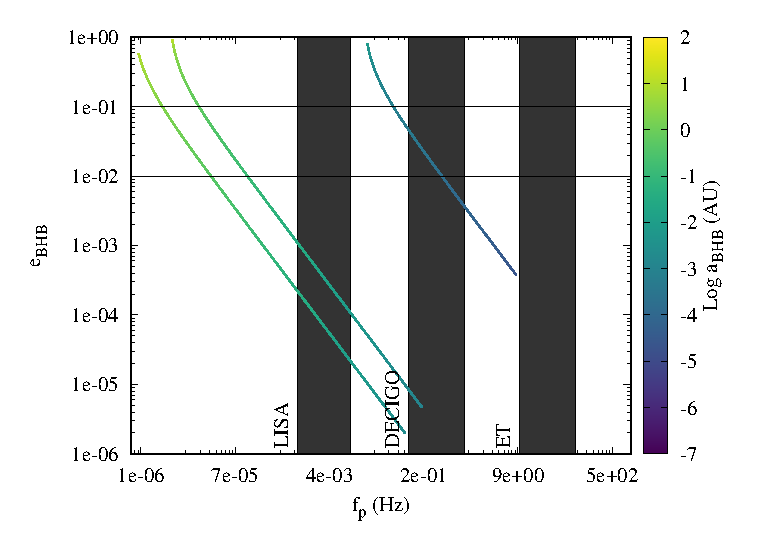
\includegraphics[width=\columnwidth]{freq_evo}\\
\caption{Frequency (x-axis) and eccentricity (y-axis) evolution for merging binaries in our models. The color coding identifies the semi-major axis evolution. Black boxes are a coarse representation of observational windows for LISA, DECIGO and the Einstein Telescope. The horizontal lines mark two values of the eccentricity, namely $e=0.01-0.1$.}
\label{F10}
\end{figure}

We find that more than $95\%$ of the sources in both models transit into the $5\times 10^{-4} - 5\times 10^{-3}$ Hz band, where LISA is sensitive. Approximately $10\%$ instead are characterized by GW emission in DHz regime, being potentially observed with LIGO and, in the future, with DECIGO and ET.
The numbers of sources appearing in different bands are summarized in Table \ref{tab:t4}.
From Table \ref{tab:t4} appears evident that the number of IMRIs entering the $> 10$ Hz band is larger than in the other two sets. This is due to the fact that, for IMBH masses $M_\ibh < 10^4\Ms$ the number of mergers in SET2 is up to two times larger, thus causing a larger number of high-frequency GW emitters.   
It is interesting to note that a handful of sources could have a non-negligible eccentricity both in the LISA and DECIGO observational band, while at larger frequencies the binaries are already completely circular. In order to better highlight the probability for low-frequency detectors to observe eccentric IMRIs, we show in Figure \ref{F11} the eccentricity distribution of sources entering the mHz and Hz frequency bands. We find that the amount of sources maintaining an eccentricity above 0.1 while transiting either the low- or high-frequency bands of GW detectors is limited to $1-5\%$, regardless of the models set.  
 
 \begin{table*}
     \centering
     \caption{Number of IMRI in different frequency bands}
     \begin{tabular}{ccccccc}
        \hline
        \hline
        model & IMRI & $N_{\rm mHz}$ & $N_{\rm cHz}$ & $N_{\rm dHz}$ & $N_{\rm Hz}$ & $N_{\rm DHz}$ \\ 
              &    total number  &$0.5-5$ mHz    & $ 0.5-5$ cHz  &  $0.5-5$ dHz & $0.5-10$ Hz & $>10$ Hz \\
        \hline
		SET0& 259 & 255 & 257 & 158 & 60  & 14 \\
		SET1& 312 & 306 & 309 & 184 & 62  & 15 \\
		SET2& 307 & 306 & 307 & 212 & 129 & 40 \\
        \hline
     \end{tabular}
     \label{tab:t4}
 \end{table*}
 
 
\begin{figure}
\centering
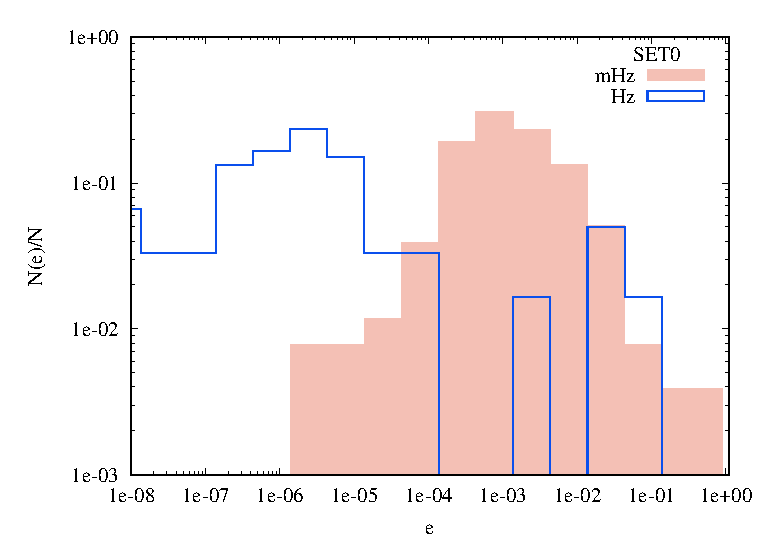
\includegraphics[width=\columnwidth]{mergers_eccen}\\
\caption{Eccentricity distribution for IMRIs in our models. The eccentricity is calculated at the moment in which a source cross the mHz (red filled steps) or Hz frequency band (black steps).}
\label{F11}
\end{figure}

In order to infer whether these sources might be audible to GW observatories, we calculated the strain following \cite{kocsis12} for all the frequencies containing the $95\%$ of the emitted power. We assume a luminosity distance $D_L = 463$ Mpc (redshift $z=0.1$), and a 4 yr observation time. Figure \ref{F12} shows the evolution of the strain-frequency evolution for two different mergers, altogether with the eccentricity decrease due to GW circularization.

For the sake of visibility, we only show the strain associated to the dominant frequency. In the two models shown in the plot, the mergers outshine in the LISA band, where they spend most of their life, and slowly shift toward higher frequency, merging inside the LIGO observational band. These sources are of extreme interest since they can be used to further constrain and test the General Relativity theory, as their evolution can be monitored in both the low- and high-frequency regime. 

\begin{figure}
\centering
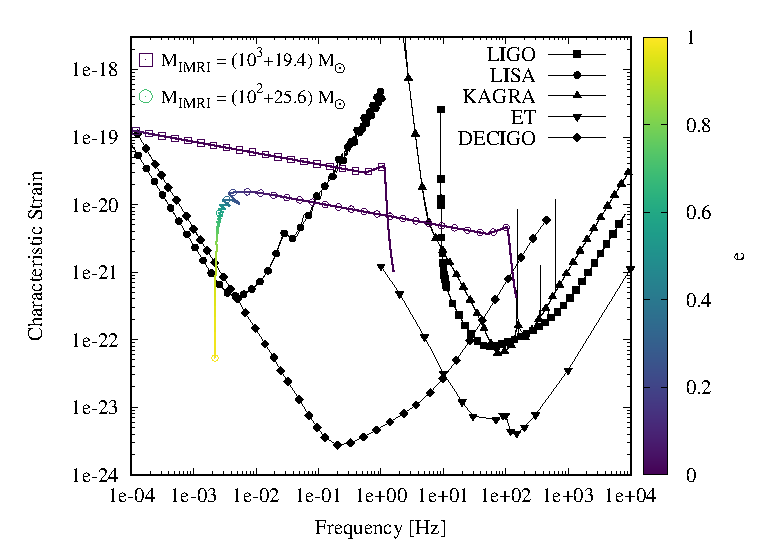
\includegraphics[width=\columnwidth]{example_signal}\\
\caption{Strain calculated for the dominant frequency for two different models, assuming an infinite observational time. We overlap the simulated data with sensitivity curves from several GW observatories.}
\label{F12}
\end{figure}

\section{Conclusions}

In this paper we presented the results of a suite of 6000 direct N-body simulations modelling the evolution of an IMBH-BH binary orbited by a third BH, taking into account post-Newtonian corrections up to order 2.5 and the gravitational field of the host cluster (treated as an external potential). The simulations are gathered into three sets: set 0 and 1 differ in the scaling relation adopted to connect the masses of the IMBH and its host cluster, whereas set 2 is similar to set 0 but we assumed a range of wider orbits for the outer BH. In all models, we vary the IMBH mass between $10^2-10^6\Ms$ with the aim to unveil the dependence between this quantity and the probability for IMRIs to form.
Our results can be summarized as follows:
\begin{itemize}
\item at formation, IMRIs formed via the IMBH-BH-BH interactions exhibit an eccentricity distribution much steeper than the initially adopted one, i.e. $N(e) \propto e^5$. The distribution of semimajor axis, instead, shows a sharp decline at values above $\sim 50$ AU and a clear cut-off at $\sim 100$ AU (Figure 3, put ref: \ref{});
\item the average eccentricity of IMRIs at formation seems to decrease with the IMBH mass, suggesting that the formation of highly eccentric IMRIs through the channel described here is favoured for IMBH masses below $10^5\Ms$ (Figure 4, put ref: \ref{});
\item merger times for this class of sources shows a steep rise toward $\sim 1-10$ Gyr, with a broad 
distribution down to $\sim 1$ yr. In all the models investigated, more than $50\%$ of IMRIs have a merger time below $0.1-1$ Gyr (Figure 5, put ref: \ref{});
\item from our simulations, we infer an IMRI formation probability of $12-15\%$, regardless of the assumptions made. This quantity increases at increasing the IMBH mass and, correspondingly, heavier GCs, following a powerlaw for IMBH masses above $10^3\Ms$ (Figure 6 - 7, put refs: \ref{});
\item in a few particular cases, we find that the two stellar BHs have orbits sufficiently similar to favour the formation of a bound pair that orbit the IMBH. The IMBH field exert on the stellar BH binary Kozai-Lidov oscillations that trigger the binary merger in $\sim 10^7$ yr, a timescale $\sim 5600$ times smaller than the merger time for the same binary in isolation (Figure 8, put ref: \ref{}). We find that the probability for these events to occur is $\sim 0.8\%$; 
\item upon simplistic assumptions, we derive an IMRI occurrence rate of $\sim 2.26\times 10^5$ yr$^{-1}$ in the MW and similar galaxies, which corresponds to $\sim 10$ yr$^{-1}$ events in the volume encompassed by a luminosity distance of $D_L = 470$ Mpc (i.e. redshift $z\leq 0.1$) (Equation 16, put ref: \ref{});
\item assuming a 4 yr observation time and a signal-to-noise ratio of 15, we calculate the horizon redshift of IMRIs for four GW detectors: LIGO, LISA, ET, DECIGO. We find that LIGO can observe IMRI with mass ratios above $0.05$ and total mass $<250\Ms$ out to redshift $z<0.6$. LISA will permit the observations of heavier IMRIs (total mass up to $10^5-10^6\Ms$) out to redshift $z=10$, but the horizon redshift will be much smaller ($z < 1$) for IMBHs with a mass $M_\ibh<10^4\Ms$. The next generation of GW telescopes has the potential to chase IMBHs and IMRIs formation much farther in time and space. ET can provide observations of IMRIs in the IMBH mass range $10^2-10^3\Ms$ out to redshift 10, whereas DECIGO can potentially probe IMRIs formation up to redshift $z > 100-1000$, well beyond the time at which the first stars formed. The possible construction of GW detectors sensitive in the dHz frequency band thus appear to be a very promising way to chase these systems up to the dawn of the Universe (Figure 9, put ref: \ref{});
\item combining our simulations, the calculated horizon redshift, and taking advantage of observational limits on the cosmological distribution of galaxies, we derive an IMRI merger rate for the four detectors discussed in the previous point and assuming a 4 yr observation time. We find that LIGO should be capable of observing up to 1-5 IMRIs per year with masses below $230\Ms$, whereas LISA could deliver up to 30 observations per yr for IMRIs with masses up to $5\times 10^4\Ms$. The next generation of detectors will definitely lead to an improvement of these numbers, being the inferred rate for ET in the range of $250-2000$ yr$^{-1}$ for IMRIs with masses below $10^3\Ms$ and for DECIGO up to $4400$ yr$^{-1}$ for IMRIs covering the whole mass range $10^2-10^5\Ms$ (Table 4, put ref: \ref{});
\item for all IMRIs in our sample, we follow the evolution of the orbital parameters down to the merger. Despite IMRIs tend to have a high eccentricity at formation, circularization due to GW emission has already took place by the time in which the source enter in the frequency range accessible by GW detectors. We find that only $\sim 1\%$ of IMRIs have a residual eccentricity above $e = 0.1$ when entering the mHz regime (Figure 11, put ref: \ref{});
\item we derive the GW strain for all IMRIs in our sample, showing that these sources has the potential to be interesting multiband sources. Once decihertz observatories will fly and third generation detectors will be operative, we could be able to observe the whole evolution of IMRIs with masses in the range $10^2-10^4\Ms$ with at least two instruments, covering both the spiralling and merger phase (Figure 12, put ref: \ref{});  
  
\end{itemize}

\section*{Acknowledgements}

Sonderforschungsbereich SFB 881 "The Milky Way System" (subproject Z2) of the
German Research Foundation (DFG) for the financial support provided. This work
benefited of financial support from the Alexander von Humboldt Foundation,
which granted MAS research program ``The evolution of black holes from stellar
to galactic scales''.  This work benefited from support by the ISSI (Bern),
through its Intern. Team prog. ref. no. 393 {\it The Evolution of Rich Stellar
Populations \& BH Binaries} (2017-18).  PAS acknowledges support from the
Ram{\'o}n y Cajal Programme of the Ministry of Economy, Industry and
Competitiveness of Spain, as well as the COST Action GWverse CA16104. This work
was supported by the National Key R\&D Program of China (2016YFA0400702) and
the National Science Foundation of China (11721303).

\footnotesize{
\bibliographystyle{mn2e}
\bibliography{aamnem99,biblio,ASetal2015}
}



\end{document}
